\DeclareUnicodeCharacter{041B}{\CYRL}



\documentclass[11pt]{article}

    
    
    \usepackage[breakable]{tcolorbox}
    \usepackage{parskip} % Stop auto-indenting (to mimic markdown behaviour)
    \usepackage[english,russian]{babel}
    \usepackage{graphicx}
    \usepackage{subcaption}
    

    % Basic figure setup, for now with no caption control since it's done
    % automatically by Pandoc (which extracts ![](path) syntax from Markdown).
    \usepackage{graphicx}
    % Maintain compatibility with old templates. Remove in nbconvert 6.0
    \let\Oldincludegraphics\includegraphics
    % Ensure that by default, figures have no caption (until we provide a
    % proper Figure object with a Caption API and a way to capture that
    % in the conversion process - todo).
    \usepackage{caption}
    \DeclareCaptionFormat{nocaption}{}
    \captionsetup{format=nocaption,aboveskip=0pt,belowskip=0pt}

    \usepackage{float}
    \floatplacement{figure}{H} % forces figures to be placed at the correct location
    \usepackage{xcolor} % Allow colors to be defined
    \usepackage{enumerate} % Needed for markdown enumerations to work
    \usepackage{geometry} % Used to adjust the document margins
    \usepackage{amsmath} % Equations
    \usepackage{amssymb} % Equations
    \usepackage{textcomp} % defines textquotesingle
    % Hack from http://tex.stackexchange.com/a/47451/13684:
    \AtBeginDocument{%
        \def\PYZsq{\textquotesingle}% Upright quotes in Pygmentized code
    }
    \usepackage{upquote} % Upright quotes for verbatim code
    \usepackage{eurosym} % defines \euro

    \usepackage{iftex}
    \ifPDFTeX
        \usepackage[T1]{fontenc}
        \IfFileExists{alphabeta.sty}{
              \usepackage{alphabeta}
          }{
              \usepackage[mathletters]{ucs}
              \usepackage[utf8x]{inputenc}
          }
    \else
        \usepackage{fontspec}
        \usepackage{unicode-math}
    \fi

    \usepackage{fancyvrb} % verbatim replacement that allows latex
    \usepackage{grffile} % extends the file name processing of package graphics
                         % to support a larger range
    \makeatletter % fix for old versions of grffile with XeLaTeX
    \@ifpackagelater{grffile}{2019/11/01}
    {
      % Do nothing on new versions
    }
    {
      \def\Gread@@xetex#1{%
        \IfFileExists{"\Gin@base".bb}%
        {\Gread@eps{\Gin@base.bb}}%
        {\Gread@@xetex@aux#1}%
      }
    }
    \makeatother
    \usepackage[Export]{adjustbox} % Used to constrain images to a maximum size
    \adjustboxset{max size={0.9\linewidth}{0.9\paperheight}}

    % The hyperref package gives us a pdf with properly built
    % internal navigation ('pdf bookmarks' for the table of contents,
    % internal cross-reference links, web links for URLs, etc.)
    \usepackage{hyperref}
    % The default LaTeX title has an obnoxious amount of whitespace. By default,
    % titling removes some of it. It also provides customization options.
    \usepackage{titling}
    \usepackage{longtable} % longtable support required by pandoc >1.10
    \usepackage{booktabs}  % table support for pandoc > 1.12.2
    \usepackage{array}     % table support for pandoc >= 2.11.3
    \usepackage{calc}      % table minipage width calculation for pandoc >= 2.11.1
    \usepackage[inline]{enumitem} % IRkernel/repr support (it uses the enumerate* environment)
    \usepackage[normalem]{ulem} % ulem is needed to support strikethroughs (\sout)
                                % normalem makes italics be italics, not underlines
    \usepackage{mathrsfs}
    

    
    % Colors for the hyperref package
    \definecolor{urlcolor}{rgb}{0,.145,.698}
    \definecolor{linkcolor}{rgb}{.71,0.21,0.01}
    \definecolor{citecolor}{rgb}{.12,.54,.11}

    % ANSI colors
    \definecolor{ansi-black}{HTML}{3E424D}
    \definecolor{ansi-black-intense}{HTML}{282C36}
    \definecolor{ansi-red}{HTML}{E75C58}
    \definecolor{ansi-red-intense}{HTML}{B22B31}
    \definecolor{ansi-green}{HTML}{00A250}
    \definecolor{ansi-green-intense}{HTML}{007427}
    \definecolor{ansi-yellow}{HTML}{DDB62B}
    \definecolor{ansi-yellow-intense}{HTML}{B27D12}
    \definecolor{ansi-blue}{HTML}{208FFB}
    \definecolor{ansi-blue-intense}{HTML}{0065CA}
    \definecolor{ansi-magenta}{HTML}{D160C4}
    \definecolor{ansi-magenta-intense}{HTML}{A03196}
    \definecolor{ansi-cyan}{HTML}{60C6C8}
    \definecolor{ansi-cyan-intense}{HTML}{258F8F}
    \definecolor{ansi-white}{HTML}{C5C1B4}
    \definecolor{ansi-white-intense}{HTML}{A1A6B2}
    \definecolor{ansi-default-inverse-fg}{HTML}{FFFFFF}
    \definecolor{ansi-default-inverse-bg}{HTML}{000000}

    % common color for the border for error outputs.
    \definecolor{outerrorbackground}{HTML}{FFDFDF}

    % commands and environments needed by pandoc snippets
    % extracted from the output of `pandoc -s`
    \providecommand{\tightlist}{%
      \setlength{\itemsep}{0pt}\setlength{\parskip}{0pt}}
    \DefineVerbatimEnvironment{Highlighting}{Verbatim}{commandchars=\\\{\}}
    % Add ',fontsize=\small' for more characters per line
    \newenvironment{Shaded}{}{}
    \newcommand{\KeywordTok}[1]{\textcolor[rgb]{0.00,0.44,0.13}{\textbf{{#1}}}}
    \newcommand{\DataTypeTok}[1]{\textcolor[rgb]{0.56,0.13,0.00}{{#1}}}
    \newcommand{\DecValTok}[1]{\textcolor[rgb]{0.25,0.63,0.44}{{#1}}}
    \newcommand{\BaseNTok}[1]{\textcolor[rgb]{0.25,0.63,0.44}{{#1}}}
    \newcommand{\FloatTok}[1]{\textcolor[rgb]{0.25,0.63,0.44}{{#1}}}
    \newcommand{\CharTok}[1]{\textcolor[rgb]{0.25,0.44,0.63}{{#1}}}
    \newcommand{\StringTok}[1]{\textcolor[rgb]{0.25,0.44,0.63}{{#1}}}
    \newcommand{\CommentTok}[1]{\textcolor[rgb]{0.38,0.63,0.69}{\textit{{#1}}}}
    \newcommand{\OtherTok}[1]{\textcolor[rgb]{0.00,0.44,0.13}{{#1}}}
    \newcommand{\AlertTok}[1]{\textcolor[rgb]{1.00,0.00,0.00}{\textbf{{#1}}}}
    \newcommand{\FunctionTok}[1]{\textcolor[rgb]{0.02,0.16,0.49}{{#1}}}
    \newcommand{\RegionMarkerTok}[1]{{#1}}
    \newcommand{\ErrorTok}[1]{\textcolor[rgb]{1.00,0.00,0.00}{\textbf{{#1}}}}
    \newcommand{\NormalTok}[1]{{#1}}

    % Additional commands for more recent versions of Pandoc
    \newcommand{\ConstantTok}[1]{\textcolor[rgb]{0.53,0.00,0.00}{{#1}}}
    \newcommand{\SpecialCharTok}[1]{\textcolor[rgb]{0.25,0.44,0.63}{{#1}}}
    \newcommand{\VerbatimStringTok}[1]{\textcolor[rgb]{0.25,0.44,0.63}{{#1}}}
    \newcommand{\SpecialStringTok}[1]{\textcolor[rgb]{0.73,0.40,0.53}{{#1}}}
    \newcommand{\ImportTok}[1]{{#1}}
    \newcommand{\DocumentationTok}[1]{\textcolor[rgb]{0.73,0.13,0.13}{\textit{{#1}}}}
    \newcommand{\AnnotationTok}[1]{\textcolor[rgb]{0.38,0.63,0.69}{\textbf{\textit{{#1}}}}}
    \newcommand{\CommentVarTok}[1]{\textcolor[rgb]{0.38,0.63,0.69}{\textbf{\textit{{#1}}}}}
    \newcommand{\VariableTok}[1]{\textcolor[rgb]{0.10,0.09,0.49}{{#1}}}
    \newcommand{\ControlFlowTok}[1]{\textcolor[rgb]{0.00,0.44,0.13}{\textbf{{#1}}}}
    \newcommand{\OperatorTok}[1]{\textcolor[rgb]{0.40,0.40,0.40}{{#1}}}
    \newcommand{\BuiltInTok}[1]{{#1}}
    \newcommand{\ExtensionTok}[1]{{#1}}
    \newcommand{\PreprocessorTok}[1]{\textcolor[rgb]{0.74,0.48,0.00}{{#1}}}
    \newcommand{\AttributeTok}[1]{\textcolor[rgb]{0.49,0.56,0.16}{{#1}}}
    \newcommand{\InformationTok}[1]{\textcolor[rgb]{0.38,0.63,0.69}{\textbf{\textit{{#1}}}}}
    \newcommand{\WarningTok}[1]{\textcolor[rgb]{0.38,0.63,0.69}{\textbf{\textit{{#1}}}}}


    % Define a nice break command that doesn't care if a line doesn't already
    % exist.
    \def\br{\hspace*{\fill} \\* }
    % Math Jax compatibility definitions
    \def\gt{>}
    \def\lt{<}
    \let\Oldtex\TeX
    \let\Oldlatex\LaTeX
    \renewcommand{\TeX}{\textrm{\Oldtex}}
    \renewcommand{\LaTeX}{\textrm{\Oldlatex}}
    % Document parameters
    % Document title
    \title{CHM\_Lab1}
    
    
    
    
    
% Pygments definitions
\makeatletter
\def\PY@reset{\let\PY@it=\relax \let\PY@bf=\relax%
    \let\PY@ul=\relax \let\PY@tc=\relax%
    \let\PY@bc=\relax \let\PY@ff=\relax}
\def\PY@tok#1{\csname PY@tok@#1\endcsname}
\def\PY@toks#1+{\ifx\relax#1\empty\else%
    \PY@tok{#1}\expandafter\PY@toks\fi}
\def\PY@do#1{\PY@bc{\PY@tc{\PY@ul{%
    \PY@it{\PY@bf{\PY@ff{#1}}}}}}}
\def\PY#1#2{\PY@reset\PY@toks#1+\relax+\PY@do{#2}}

\@namedef{PY@tok@w}{\def\PY@tc##1{\textcolor[rgb]{0.73,0.73,0.73}{##1}}}
\@namedef{PY@tok@c}{\let\PY@it=\textit\def\PY@tc##1{\textcolor[rgb]{0.24,0.48,0.48}{##1}}}
\@namedef{PY@tok@cp}{\def\PY@tc##1{\textcolor[rgb]{0.61,0.40,0.00}{##1}}}
\@namedef{PY@tok@k}{\let\PY@bf=\textbf\def\PY@tc##1{\textcolor[rgb]{0.00,0.50,0.00}{##1}}}
\@namedef{PY@tok@kp}{\def\PY@tc##1{\textcolor[rgb]{0.00,0.50,0.00}{##1}}}
\@namedef{PY@tok@kt}{\def\PY@tc##1{\textcolor[rgb]{0.69,0.00,0.25}{##1}}}
\@namedef{PY@tok@o}{\def\PY@tc##1{\textcolor[rgb]{0.40,0.40,0.40}{##1}}}
\@namedef{PY@tok@ow}{\let\PY@bf=\textbf\def\PY@tc##1{\textcolor[rgb]{0.67,0.13,1.00}{##1}}}
\@namedef{PY@tok@nb}{\def\PY@tc##1{\textcolor[rgb]{0.00,0.50,0.00}{##1}}}
\@namedef{PY@tok@nf}{\def\PY@tc##1{\textcolor[rgb]{0.00,0.00,1.00}{##1}}}
\@namedef{PY@tok@nc}{\let\PY@bf=\textbf\def\PY@tc##1{\textcolor[rgb]{0.00,0.00,1.00}{##1}}}
\@namedef{PY@tok@nn}{\let\PY@bf=\textbf\def\PY@tc##1{\textcolor[rgb]{0.00,0.00,1.00}{##1}}}
\@namedef{PY@tok@ne}{\let\PY@bf=\textbf\def\PY@tc##1{\textcolor[rgb]{0.80,0.25,0.22}{##1}}}
\@namedef{PY@tok@nv}{\def\PY@tc##1{\textcolor[rgb]{0.10,0.09,0.49}{##1}}}
\@namedef{PY@tok@no}{\def\PY@tc##1{\textcolor[rgb]{0.53,0.00,0.00}{##1}}}
\@namedef{PY@tok@nl}{\def\PY@tc##1{\textcolor[rgb]{0.46,0.46,0.00}{##1}}}
\@namedef{PY@tok@ni}{\let\PY@bf=\textbf\def\PY@tc##1{\textcolor[rgb]{0.44,0.44,0.44}{##1}}}
\@namedef{PY@tok@na}{\def\PY@tc##1{\textcolor[rgb]{0.41,0.47,0.13}{##1}}}
\@namedef{PY@tok@nt}{\let\PY@bf=\textbf\def\PY@tc##1{\textcolor[rgb]{0.00,0.50,0.00}{##1}}}
\@namedef{PY@tok@nd}{\def\PY@tc##1{\textcolor[rgb]{0.67,0.13,1.00}{##1}}}
\@namedef{PY@tok@s}{\def\PY@tc##1{\textcolor[rgb]{0.73,0.13,0.13}{##1}}}
\@namedef{PY@tok@sd}{\let\PY@it=\textit\def\PY@tc##1{\textcolor[rgb]{0.73,0.13,0.13}{##1}}}
\@namedef{PY@tok@si}{\let\PY@bf=\textbf\def\PY@tc##1{\textcolor[rgb]{0.64,0.35,0.47}{##1}}}
\@namedef{PY@tok@se}{\let\PY@bf=\textbf\def\PY@tc##1{\textcolor[rgb]{0.67,0.36,0.12}{##1}}}
\@namedef{PY@tok@sr}{\def\PY@tc##1{\textcolor[rgb]{0.64,0.35,0.47}{##1}}}
\@namedef{PY@tok@ss}{\def\PY@tc##1{\textcolor[rgb]{0.10,0.09,0.49}{##1}}}
\@namedef{PY@tok@sx}{\def\PY@tc##1{\textcolor[rgb]{0.00,0.50,0.00}{##1}}}
\@namedef{PY@tok@m}{\def\PY@tc##1{\textcolor[rgb]{0.40,0.40,0.40}{##1}}}
\@namedef{PY@tok@gh}{\let\PY@bf=\textbf\def\PY@tc##1{\textcolor[rgb]{0.00,0.00,0.50}{##1}}}
\@namedef{PY@tok@gu}{\let\PY@bf=\textbf\def\PY@tc##1{\textcolor[rgb]{0.50,0.00,0.50}{##1}}}
\@namedef{PY@tok@gd}{\def\PY@tc##1{\textcolor[rgb]{0.63,0.00,0.00}{##1}}}
\@namedef{PY@tok@gi}{\def\PY@tc##1{\textcolor[rgb]{0.00,0.52,0.00}{##1}}}
\@namedef{PY@tok@gr}{\def\PY@tc##1{\textcolor[rgb]{0.89,0.00,0.00}{##1}}}
\@namedef{PY@tok@ge}{\let\PY@it=\textit}
\@namedef{PY@tok@gs}{\let\PY@bf=\textbf}
\@namedef{PY@tok@gp}{\let\PY@bf=\textbf\def\PY@tc##1{\textcolor[rgb]{0.00,0.00,0.50}{##1}}}
\@namedef{PY@tok@go}{\def\PY@tc##1{\textcolor[rgb]{0.44,0.44,0.44}{##1}}}
\@namedef{PY@tok@gt}{\def\PY@tc##1{\textcolor[rgb]{0.00,0.27,0.87}{##1}}}
\@namedef{PY@tok@err}{\def\PY@bc##1{{\setlength{\fboxsep}{\string -\fboxrule}\fcolorbox[rgb]{1.00,0.00,0.00}{1,1,1}{\strut ##1}}}}
\@namedef{PY@tok@kc}{\let\PY@bf=\textbf\def\PY@tc##1{\textcolor[rgb]{0.00,0.50,0.00}{##1}}}
\@namedef{PY@tok@kd}{\let\PY@bf=\textbf\def\PY@tc##1{\textcolor[rgb]{0.00,0.50,0.00}{##1}}}
\@namedef{PY@tok@kn}{\let\PY@bf=\textbf\def\PY@tc##1{\textcolor[rgb]{0.00,0.50,0.00}{##1}}}
\@namedef{PY@tok@kr}{\let\PY@bf=\textbf\def\PY@tc##1{\textcolor[rgb]{0.00,0.50,0.00}{##1}}}
\@namedef{PY@tok@bp}{\def\PY@tc##1{\textcolor[rgb]{0.00,0.50,0.00}{##1}}}
\@namedef{PY@tok@fm}{\def\PY@tc##1{\textcolor[rgb]{0.00,0.00,1.00}{##1}}}
\@namedef{PY@tok@vc}{\def\PY@tc##1{\textcolor[rgb]{0.10,0.09,0.49}{##1}}}
\@namedef{PY@tok@vg}{\def\PY@tc##1{\textcolor[rgb]{0.10,0.09,0.49}{##1}}}
\@namedef{PY@tok@vi}{\def\PY@tc##1{\textcolor[rgb]{0.10,0.09,0.49}{##1}}}
\@namedef{PY@tok@vm}{\def\PY@tc##1{\textcolor[rgb]{0.10,0.09,0.49}{##1}}}
\@namedef{PY@tok@sa}{\def\PY@tc##1{\textcolor[rgb]{0.73,0.13,0.13}{##1}}}
\@namedef{PY@tok@sb}{\def\PY@tc##1{\textcolor[rgb]{0.73,0.13,0.13}{##1}}}
\@namedef{PY@tok@sc}{\def\PY@tc##1{\textcolor[rgb]{0.73,0.13,0.13}{##1}}}
\@namedef{PY@tok@dl}{\def\PY@tc##1{\textcolor[rgb]{0.73,0.13,0.13}{##1}}}
\@namedef{PY@tok@s2}{\def\PY@tc##1{\textcolor[rgb]{0.73,0.13,0.13}{##1}}}
\@namedef{PY@tok@sh}{\def\PY@tc##1{\textcolor[rgb]{0.73,0.13,0.13}{##1}}}
\@namedef{PY@tok@s1}{\def\PY@tc##1{\textcolor[rgb]{0.73,0.13,0.13}{##1}}}
\@namedef{PY@tok@mb}{\def\PY@tc##1{\textcolor[rgb]{0.40,0.40,0.40}{##1}}}
\@namedef{PY@tok@mf}{\def\PY@tc##1{\textcolor[rgb]{0.40,0.40,0.40}{##1}}}
\@namedef{PY@tok@mh}{\def\PY@tc##1{\textcolor[rgb]{0.40,0.40,0.40}{##1}}}
\@namedef{PY@tok@mi}{\def\PY@tc##1{\textcolor[rgb]{0.40,0.40,0.40}{##1}}}
\@namedef{PY@tok@il}{\def\PY@tc##1{\textcolor[rgb]{0.40,0.40,0.40}{##1}}}
\@namedef{PY@tok@mo}{\def\PY@tc##1{\textcolor[rgb]{0.40,0.40,0.40}{##1}}}
\@namedef{PY@tok@ch}{\let\PY@it=\textit\def\PY@tc##1{\textcolor[rgb]{0.24,0.48,0.48}{##1}}}
\@namedef{PY@tok@cm}{\let\PY@it=\textit\def\PY@tc##1{\textcolor[rgb]{0.24,0.48,0.48}{##1}}}
\@namedef{PY@tok@cpf}{\let\PY@it=\textit\def\PY@tc##1{\textcolor[rgb]{0.24,0.48,0.48}{##1}}}
\@namedef{PY@tok@c1}{\let\PY@it=\textit\def\PY@tc##1{\textcolor[rgb]{0.24,0.48,0.48}{##1}}}
\@namedef{PY@tok@cs}{\let\PY@it=\textit\def\PY@tc##1{\textcolor[rgb]{0.24,0.48,0.48}{##1}}}

\def\PYZbs{\char`\\}
\def\PYZus{\char`\_}
\def\PYZob{\char`\{}
\def\PYZcb{\char`\}}
\def\PYZca{\char`\^}
\def\PYZam{\char`\&}
\def\PYZlt{\char`\<}
\def\PYZgt{\char`\>}
\def\PYZsh{\char`\#}
\def\PYZpc{\char`\%}
\def\PYZdl{\char`\$}
\def\PYZhy{\char`\-}
\def\PYZsq{\char`\'}
\def\PYZdq{\char`\"}
\def\PYZti{\char`\~}
% for compatibility with earlier versions
\def\PYZat{@}
\def\PYZlb{[}
\def\PYZrb{]}
\makeatother


    % For linebreaks inside Verbatim environment from package fancyvrb.
    \makeatletter
        \newbox\Wrappedcontinuationbox
        \newbox\Wrappedvisiblespacebox
        \newcommand*\Wrappedvisiblespace {\textcolor{red}{\textvisiblespace}}
        \newcommand*\Wrappedcontinuationsymbol {\textcolor{red}{\llap{\tiny$\m@th\hookrightarrow$}}}
        \newcommand*\Wrappedcontinuationindent {3ex }
        \newcommand*\Wrappedafterbreak {\kern\Wrappedcontinuationindent\copy\Wrappedcontinuationbox}
        % Take advantage of the already applied Pygments mark-up to insert
        % potential linebreaks for TeX processing.
        %        {, <, #, %, $, ' and ": go to next line.
        %        _, }, ^, &, >, - and ~: stay at end of broken line.
        % Use of \textquotesingle for straight quote.
        \newcommand*\Wrappedbreaksatspecials {%
            \def\PYGZus{\discretionary{\char`\_}{\Wrappedafterbreak}{\char`\_}}%
            \def\PYGZob{\discretionary{}{\Wrappedafterbreak\char`\{}{\char`\{}}%
            \def\PYGZcb{\discretionary{\char`\}}{\Wrappedafterbreak}{\char`\}}}%
            \def\PYGZca{\discretionary{\char`\^}{\Wrappedafterbreak}{\char`\^}}%
            \def\PYGZam{\discretionary{\char`\&}{\Wrappedafterbreak}{\char`\&}}%
            \def\PYGZlt{\discretionary{}{\Wrappedafterbreak\char`\<}{\char`\<}}%
            \def\PYGZgt{\discretionary{\char`\>}{\Wrappedafterbreak}{\char`\>}}%
            \def\PYGZsh{\discretionary{}{\Wrappedafterbreak\char`\#}{\char`\#}}%
            \def\PYGZpc{\discretionary{}{\Wrappedafterbreak\char`\%}{\char`\%}}%
            \def\PYGZdl{\discretionary{}{\Wrappedafterbreak\char`\$}{\char`\$}}%
            \def\PYGZhy{\discretionary{\char`\-}{\Wrappedafterbreak}{\char`\-}}%
            \def\PYGZsq{\discretionary{}{\Wrappedafterbreak\textquotesingle}{\textquotesingle}}%
            \def\PYGZdq{\discretionary{}{\Wrappedafterbreak\char`\"}{\char`\"}}%
            \def\PYGZti{\discretionary{\char`\~}{\Wrappedafterbreak}{\char`\~}}%
        }
        % Some characters . , ; ? ! / are not pygmentized.
        % This macro makes them "active" and they will insert potential linebreaks
        \newcommand*\Wrappedbreaksatpunct {%
            \lccode`\~`\.\lowercase{\def~}{\discretionary{\hbox{\char`\.}}{\Wrappedafterbreak}{\hbox{\char`\.}}}%
            \lccode`\~`\,\lowercase{\def~}{\discretionary{\hbox{\char`\,}}{\Wrappedafterbreak}{\hbox{\char`\,}}}%
            \lccode`\~`\;\lowercase{\def~}{\discretionary{\hbox{\char`\;}}{\Wrappedafterbreak}{\hbox{\char`\;}}}%
            \lccode`\~`\:\lowercase{\def~}{\discretionary{\hbox{\char`\:}}{\Wrappedafterbreak}{\hbox{\char`\:}}}%
            \lccode`\~`\?\lowercase{\def~}{\discretionary{\hbox{\char`\?}}{\Wrappedafterbreak}{\hbox{\char`\?}}}%
            \lccode`\~`\!\lowercase{\def~}{\discretionary{\hbox{\char`\!}}{\Wrappedafterbreak}{\hbox{\char`\!}}}%
            \lccode`\~`\/\lowercase{\def~}{\discretionary{\hbox{\char`\/}}{\Wrappedafterbreak}{\hbox{\char`\/}}}%
            \catcode`\.\active
            \catcode`\,\active
            \catcode`\;\active
            \catcode`\:\active
            \catcode`\?\active
            \catcode`\!\active
            \catcode`\/\active
            \lccode`\~`\~
        }
    \makeatother

    \let\OriginalVerbatim=\Verbatim
    \makeatletter
    \renewcommand{\Verbatim}[1][1]{%
        %\parskip\z@skip
        \sbox\Wrappedcontinuationbox {\Wrappedcontinuationsymbol}%
        \sbox\Wrappedvisiblespacebox {\FV@SetupFont\Wrappedvisiblespace}%
        \def\FancyVerbFormatLine ##1{\hsize\linewidth
            \vtop{\raggedright\hyphenpenalty\z@\exhyphenpenalty\z@
                \doublehyphendemerits\z@\finalhyphendemerits\z@
                \strut ##1\strut}%
        }%
        % If the linebreak is at a space, the latter will be displayed as visible
        % space at end of first line, and a continuation symbol starts next line.
        % Stretch/shrink are however usually zero for typewriter font.
        \def\FV@Space {%
            \nobreak\hskip\z@ plus\fontdimen3\font minus\fontdimen4\font
            \discretionary{\copy\Wrappedvisiblespacebox}{\Wrappedafterbreak}
            {\kern\fontdimen2\font}%
        }%

        % Allow breaks at special characters using \PYG... macros.
        \Wrappedbreaksatspecials
        % Breaks at punctuation characters . , ; ? ! and / need catcode=\active
        \OriginalVerbatim[#1,codes*=\Wrappedbreaksatpunct]%
    }
    \makeatother

    % Exact colors from NB
    \definecolor{incolor}{HTML}{303F9F}
    \definecolor{outcolor}{HTML}{D84315}
    \definecolor{cellborder}{HTML}{CFCFCF}
    \definecolor{cellbackground}{HTML}{F7F7F7}

    % prompt
    \makeatletter
    \newcommand{\boxspacing}{\kern\kvtcb@left@rule\kern\kvtcb@boxsep}
    \makeatother
    \newcommand{\prompt}[4]{
        {\ttfamily\llap{{\color{#2}[#3]:\hspace{3pt}#4}}\vspace{-\baselineskip}}
    }
    

    
    % Prevent overflowing lines due to hard-to-break entities
    \sloppy
    % Setup hyperref package
    \hypersetup{
      breaklinks=true,  % so long urls are correctly broken across lines
      colorlinks=true,
      urlcolor=urlcolor,
      linkcolor=linkcolor,
      citecolor=citecolor,
      }
    % Slightly bigger margins than the latex defaults
    
    \geometry{verbose,tmargin=1in,bmargin=1in,lmargin=1in,rmargin=1in}
    
\newtheorem{theorem}{Теорема}

\begin{document}
    
    \begin{titlepage}
    \newpage
    
    \begin{center}
    МИНИСТЕРСТВО ОБРАЗОВАНИЯ РЕСПУБЛИКИ БЕЛАРУСЬ БЕЛОРУССКИЙ ГОСУДАРСТВЕННЫЙ УНИВЕРСИТЕТ \\
    Факультет прикладной математики и инворматики \\ Кафедра вычислительной математики
 
    \end{center}
    
    \vspace{8em}
    
    \vspace{2em}
    
    \begin{center}
    \textsc{\textbf{Отчет по лабораторной работе 2 \\ "Разностные схемы для обыкновенного дифференциального уравнения второго порядка." \linebreak Вариант 5}}
    \end{center}
    
    \vspace{6em}
    
    \begin{flushright}
        Выполнил:\\
        Карпович Артём Дмитриевич\\
        студент 4 курса 7 группы
    \end{flushright}
    
    \begin{flushright}
        Преподаватель:\\
        Репников Василий Иванович
    \end{flushright}
    
    \vspace{\fill}
    
    \vspace{\fill}
    
    \begin{center}
    Минск, 2024
    \end{center}
    
    \end{titlepage}
    

    \section*{Постановка
задач}\label{ux43fux43eux441ux442ux430ux43dux43eux432ux43aux430-ux437ux430ux434ux430ux447}
\begin{enumerate}
    \item Построить разностную схему, заменяя дифференциальные производные разностными.
    \item Методом баланса построить консервативную разностную схему.
    $$1,2.\begin{cases}
        \frac{d^2u}{dx^2}-q(x)u=-f(x),\ 0<x<1,\\
        u(0)=A,\\
        u(1)=B.
    \end{cases}$$
    \item Построить вариационно-разностную схему методом наименьших квадратов.
   
    \item Используя метод разностной прогонки, составить программу решения исходной задачи с помощью разностных схем п.п. 1.-2., выполнить контрольные расчеты на ЭВМ и провести сравнительный анализ результатов.
     $$q(x)=\frac{7}{(x+1)^2}; f(x)=x+1;$$
     $$A=1;B=8.$$
     точное решение $u(x)=(x+1)^3.$
\end{enumerate}

\newpage

\subsection*{Задача 1}
\textbf{Постановка задачи.} Построить разностную схему, заменяя дифференциальные производные разностными.
    $$\begin{cases}
        \frac{d^2u}{dx^2}-q(x)u=-f(x),\ 0<x<1,\\
        u(0)=A,\\
        u(1)=B,
    \end{cases}$$
где $q(x)=\frac{7}{(x+1)^2};\ f(x)=x+1;\ A=1;\ B=8.$ Точное решение $u(x)=(x+1)^3.$
     
\textbf{Решение задачи.} В данном случае мы имеем краевую задачу для обыкновенного дифференциального уравнения второго порядка с уравнением
$$Lu(x)=\frac{d^2u}{dx^2}-q(x)u=-f(x).$$
Выберем равномерную сетку $\overline{\omega_h}=\{x_h=i\cdot h; i=\overline{0,N};h=\frac{1}{N}\}$ и рассмотрим на ней трехточечный шаблон $\{x_{i-1},x_i,x_{i+1} \}$. Тогда мы можем построить двухпараметрчиеское семейство разностных аппроксимаций:
$$L_hy(x_i)=\frac{y_{i+1}-2y_i+y_{i-1}}{h^2}-q(x_i)y_i=-f(x_i),$$

Таким образом, разностная схема в индексной форме примет вид:
$$\begin{cases}
    \frac{y_{i+1}-2y_i+y_{i-1}}{h^2}-q(x_i)y_i=-f(x_i),\\
    y_0=A,\\
    y_N=B.
\end{cases}$$
Исследуем порядок аппроксимации построенной разностной схемы, для этого рассмотрим погорешность аппроксимации дифференциального уравнения:
$$\psi_h(x)=u_{\overline{x}x}-q(x)u(x)+f(x),$$
разложим производные в ряд Тейлора:
$$u_{\overline{x}x}=u''+\frac{h^2}{12}u^{(\text{IV})}+O(h^3).$$
Тогда
$$\psi_h(x)=u''+\frac{h^2}{12}u^{(\text{IV})}-q(x)u(x)+f(x)+O(h^3)=O(h^2).$$
Таким образом, аппроксимация дифференциального уравнения имеет второй порядок.
Рассмотрим теперь аппроксимацию граничных условий. Поскольку ни в одном из граничных условий нет производных, то каждое из них аппроксимируется точно, то есть:
$$\begin{cases}
    \nu_h(0)=u(0)-A=0,\\
    \nu_h(1)=u(1)-B=0.
\end{cases}$$
Таким образом, разностная схема примет вид:
$$\begin{cases}
    \frac{y_{i+1}-2y_i+y_{i-1}}{h^2}-q(x_i)y_i=-f(x_i),\\
    y_0=u_0,\\
    y_N=u_1.
\end{cases}$$
В итоге получаем, что полученная разностная схема имеет второй порядок аппроксимации. Поскольку порядок аппроксимации дифференциального уравнения никак не был понижен граничными условиями, то и повысить порядок мы не можем.

Докажем сходимость метода прогонки для полученной разностной схемы. Для выполнение метода прогонки нам необходимо выписать коэффициенты для трехдиагнольный матрицы вида:
	\begin{equation}
		\begin{pmatrix} 
			\gamma_0 & \beta_0 & 0 & \ldots & 0 & 0 & \vrule & g_0 \\ 
			\alpha_1 & \gamma_1 & \beta_1 & \ldots & 0 & 0 & \vrule & g_1\\ 
			0 & \alpha_1 & \gamma_2 & \ldots & 0 & 0 & \vrule & g_2\\ 
			\vdots & \vdots & \vdots & \ddots & \vdots & \vdots & \vrule & \vdots\\ 
			0 & 0 & 0 & \ldots& \gamma_{N-1} & \beta_{N-1} & \vrule & g_{N-1} \\ 
			0 & 0 & 0 & \ldots& \alpha_N& \gamma_N & \vrule & g_N\\\end{pmatrix}
	\end{equation}
 Из нашей схемы получим
$$a_0=0,\ c_0=1,\ b_0=0,\ g_0=u_0,$$
$$a_i=\frac{1}{h^2},\ c_i=-\frac{2}{h^2}-q(x_i),\ b_i=\frac{1}{h^2},\ g_i=-f(x_i),$$
$$a_N=0,\ c_N=1,\ b_N=0,\ g_N=u_1.$$
Проверим выполнение условий сходимости:
$$|c_0|\geq |a_0|+|b_0| \Rightarrow 1 \geq 0 \Rightarrow \textit{Выполняется}.$$
$$|c_i|\geq |a_i| + |b_i| \Rightarrow |-\frac{2}{h^2}-q(x_i)|>\frac{2}{h^2} \Rightarrow \frac{7}{(x_i+1)^2} > 0 \Rightarrow \textit{Выполняется}.$$
$$|c_N|\geq |a_N|+|b_N| \Rightarrow 1 \geq 0 \Rightarrow \textit{Выполняется}.$$
Таким образом, получаем, что условия сходимости метода прогонки выполняются, что позволяет нам его применить.

Для реализации метода прогонки воспользуемся следующими формулами для вычисления коэффициентов
\newpage

\subsection*{Задача 2}
\textbf{Постановка задачи}. Методом баланса построить консервативную разностную схему.
    $$\begin{cases}
        \frac{d^2u}{dx^2}-q(x)u(x)=-f(x),\ 0<x<1,\\
        u(0)=A,\\
        u(1)=B,
    \end{cases}$$
где $q(x)=\frac{7}{(x+1)^2};\ f(x)=x+1;\ A=1;\ B=8.$ Точное решение $u(x)=(x+1)^3.$

\textbf{Решение задачи.} 
Для использования метода баланса необходимо привести рассматриваемую задачу к виду:
$$\begin{cases}
    (k(x)u'(x))'-q(x)u(x)=-f(x),\ 0<x<1,\\
    u(0)=\mu_0,\\
    u(1)=\mu_1.
\end{cases}$$
Рассмотрим сначала дифференциальное уравнение:
$$(k(x)u'(x))'-q(x)u(x)=-f(x),$$
раскроем первое слагаемое:
$$(k(x)u'(x))' = k'(x)u'(x)+k(x)u''(x) = u''(x).$$
Отсюда следует, что $k(x)=1.$
Воспользуемся ранее построенной разностной схемой $\overline{\omega_h},$ тогда разностная схема, полученная методом баланса, в безиндексной форме примет вид:
$$\begin{cases}
    (ay_{\overline{x}})_x-dy=-\varphi,\ x\in \omega_h,\\
    y_0=u_0,\\
    y_N=u_1,
\end{cases}$$
или в индексной форме:
$$\begin{cases}
    \frac{1}{h}\Bigl(a_{i+1}\frac{y_{i+1}-y_i}{h}-a_i\frac{y_i-y_{i-1}}{h}\Bigr)-d_iy_i=-\varphi_i,\ i=\overline{1, N-1},\\
    y_0=u_0,\\
    y_N=u_1,
\end{cases}$$
где коэффициенты сразу определим с учетом входных данных:
$$a_i=\Bigr[ \frac{1}{h} \int_{x_{i-1}}^{x_{i}} \frac{1}{k(x)}dx \Bigl]^{-1}=\Bigr[ \frac{1}{h} \int_{x_{i-1}}^{x_{i}} dx \Bigl]^{-1}=\frac{x_i-x_{i-1}}{h}=\frac{ih-(i-1)h}{h}=1,$$

$$d_i=\frac{1}{h}  \int_{x_{i-\frac{1}{2}}}^{x_{i+\frac{1}{2}}} q(x)dx=\frac{1}{h}  \int_{x_{i-\frac{1}{2}}}^{x_{i+\frac{1}{2}}} \frac{7}{(x+1)^2}dx=\frac{7}{h}  \int_{x_{i-\frac{1}{2}}}^{x_{i+\frac{1}{2}}} \frac{1}{(x+1)^2}dx=-\frac{7}{h}  \frac{1}{(x+1)}|_{x_{i-\frac{1}{2}}}^{x_{i+\frac{1}{2}}}=$$$$=-\frac{7}{h}\Bigl(\frac{1}{x_{i+\frac{1}{2}}+1}-\frac{1}{x_{i-\frac{1}{2}}+1} \Bigr)=-\frac{7}{h}\Bigl(\frac{x_{i-\frac{1}{2}} - x_{i+\frac{1}{2}}}{(x_{i+\frac{1}{2}}+1)(x_{i-\frac{1}{2}}+1)} \Bigr),$$\
$$\varphi_i(x)=\frac{1}{h} \int_{x_{i-\frac{1}{2}}}^{x_{i+\frac{1}{2}}} f(x)dx=\frac{1}{h}\int_{x_{i-\frac{1}{2}}}^{x_{i+\frac{1}{2}}} (1+x)dx=\frac{1}{h}(x+\frac{x^2}{2})|_{x_{i-\frac{1}{2}}}^{x_{i+\frac{1}{2}}}=\frac{1}{h}\Bigl( x_{i-\frac{1}{2}}-x_{i+\frac{1}{2}}+\frac{(x_{i-\frac{1}{2}})^2-(x_{i+\frac{1}{2}})^2}{2} \Bigr).$$
Таким образом, учитывая нашу задачу, разностная схема для нее, полученная методом баланса, примет вид:
$$\begin{cases}
    \frac{1}{h}\Bigl(a_{i+1}\frac{y_{i+1}-y_i}{h}-a_i\frac{y_i-y_{i-1}}{h}\Bigr)-d_iy_i=-\varphi_i,\ i=\overline{1, N-1},\\
    y_0=u_0,\\
    y_N=u_1,
\end{cases}$$
в которой мы исключили аппроксимацию граничных условий, поскольку они вычисляются точно. 

Таким образом, мы имеем общую формулу для итераций и явные выражения для коэффициентов из этой разностной схемы. 

Данная схема имеет второй порядок аппроксимации, а также для нее сходится метод прогонки, коэффициенты которого имеют вид:
$$\alpha_0=0,\ \gamma_0=1,\ \beta_0=0,\ g_0=u_0,$$
$$\alpha_i=\frac{a_i}{h^2},\ \gamma_i=-\frac{a_{i+1}+a_{i}}{h^2}-d_i,\ \beta_i=\frac{a_{i+1}}{h^2},\ g_i=-\varphi_i,$$
$$\alpha_N=0,\ \gamma_N=1,\ \beta_N=0,\ g_N=u_1.$$
Если подставить вычисленные ранее коэффициенты, то получим
$$\alpha_0=0,\ \gamma_0=1,\ \beta_0=0,\ g_0=A,$$
$$\alpha_i=\frac{1}{h^2},\ \gamma_i=-\frac{2}{h^2}+\frac{7}{h}\Bigl(\frac{x_{i-\frac{1}{2}} - x_{i+\frac{1}{2}}}{(x_{i+\frac{1}{2}}+1)(x_{i-\frac{1}{2}}+1)} \Bigr),\ \beta_i=\frac{1}{h^2},\ g_i=-\frac{1}{h}\Bigl( x_{i-\frac{1}{2}}-x_{i+\frac{1}{2}}+\frac{(x_{i-\frac{1}{2}})^2-(x_{i+\frac{1}{2}})^2}{2} \Bigr),$$
$$\alpha_N=0,\ \gamma_N=1,\ \beta_N=0,\ g_N=B.$$
\newpage
\subsection*{Задача 3}
\textbf{Постановка задачи.} Построить вариационно-разностную схему методом наименьших квадратов.

\textit{Заменено.} Построить вариационно-разностную схему методом Ритца.

\textbf{Решение.} Вернемся к нашей равномерной сетке узлов $\overline{\omega_h}$. По методу Ритца мы можем построить трехдиагональную систему вида

$$\begin{cases}
	\alpha_{ii-1} y_{i-1} + \alpha_{ii} y_i + \alpha_{i i+1} y_{i+1} = \beta_i,\ i = \overline {1, N -1},\\
	\alpha_{00} y_0 + \alpha_{01}y_1 = \beta_0,\\
	\alpha_{NN-1} y_{N-1} + \alpha_{NN}y_N = \beta_N,
\end{cases}$$
где 
$$\alpha_{ii} = \dfrac{1}{h^2}\left[ \int\limits_{x_{i-1}}^{x_{i+1}} k(x)dx +\int\limits_{x_{i-1}}^{x_i}q(x)(x-x_{i-1})^2dx + \int\limits_{x_i}^{x_{i+1}}q(x)(x_{i+1}-x)^2dx \right],\ i = \overline{1, N-1},$$
	$$\alpha_{ii+1} = \dfrac{1}{h^2} \left[-\int\limits_{x_i}^{x_{i+1}}k(x)dx + \int\limits_{x_i}^{x_{i+1}}q(x)(x-x_i)(x_{i+1} - x)dx\right],\ i = \overline {0, N-1},$$
 причем $\alpha_{ii+1}=\alpha_{i+1i}$. Тогда можно вычислить
 $$\beta_i = \dfrac{1}{h} \left[\int\limits_{x_{i-1}}^{x_i}f(x)(x-x_{i-1})dx + \int\limits_{x_i}^{x_{i+1}}f(x)(x_{i+1}-x)dx\right],\ i = \overline{1, N-1},$$
	$$\alpha_{00} = \dfrac{1}{h^2}\left[\int\limits_0^h k(x)dx + \int\limits_0^h q(x)(x-h)^2dx\right] + \sigma_1,$$
	$$\alpha_{NN} = \dfrac{1}{h^2}\left[\int\limits_{1-h}^h k(x)dx + \int\limits_{1-h}^h q(x)(x-1+h)^2dx\right] + \sigma_2,$$
	$$\beta_0 = \dfrac 1h \left[\int\limits_0^h f(x)(h-x)dx + \mu_1\right],\ \beta_N =  \dfrac{1}{h} \left[\int\limits_{1-h}^1 f(x)(x-1+h)dx + \mu_2\right].$$
 Систему, выписанную ранее можно привести к виду разностной схемы, полученной методом баланса, при этом у нас получится следующее соотношение между коэффициентами:
 $$a_i=-h\alpha_{ii-1},\ d_i=\frac{1}{h}(\alpha_{ii-1}+\alpha_{ii}+\alpha_{ii+1},\ \varphi_i=\frac{1}{h}\beta_i,\ i=\overline{1,N-1}.$$
 Тогда для нашей задачи получим разностную схему следующего вида:
$$\begin{cases}
	\dfrac{a_i}{h^2}y_{i-1} - \left(\dfrac{a_i +a_{i+1}}{h}+d_i\right)y_i + \dfrac{a_{i+1}}{h^2}y_{i+1} = -\varphi_i,\ i=\overline {1,N-1}\\
	y_0 = u_0,\\
	y_N=u_1.
\end{cases}$$
Выпишем коэффициенты для нашей задачи:
$$\alpha_{ii}=\dfrac{1}{h^2}\left[ \int\limits_{x_{i-1}}^{x_{i+1}}dx +\int\limits_{x_{i-1}}^{x_i}\frac{7}{(x+1)^2}(x-x_{i-1})^2dx + \int\limits_{x_i}^{x_{i+1}}\frac{7}{(x+1)^2}(x_{i+1}-x)^2dx \right]=$$$$=-\dfrac{1}{h}\Bigl[ 2h -7\Bigl(\Bigr( \frac{(x_{i-1}+1)^2}{x+1}-2 (x_{i-1}+1) \ln(x+1)+x\Bigl)\Big|_{x_{i-1}}^{x_i}+ $$$$ +\Bigr( \frac{(x_{i+1}+1)^2}{x+1}-2 (x_{i+1}+1) \ln(x+1)+x\Bigl)\Big|_{x_i}^{x_{i+1}}\Bigr) \Bigr],$$
$$\alpha_{ii+1} = \dfrac{1}{h^2} \left[-h + 7\left(\frac{(x_i+1) (x_{i+1}+1)}{x+1}+\ln(x+1) (x_i+x_{i+1}+2)-x\right)\Big|_{x_i}^{x_{i+1}}\right],$$
$$\alpha_{ii-1} = \dfrac{1}{h^2} \left[-h + 7\left(\frac{(x_i+1) (x_{i-1}+1)}{x+1}+\ln(x+1) (x_i+x_{i-1}+2)-x\right)\Big|_{x_{i-1}}^{x_{i}}\right],$$
$$\beta_i = \dfrac{1}{h} \left[\int\limits_{x_{i-1}}^{x_i}(x+1)(x-x_{i-1})dx + \int\limits_{x_i}^{x_{i+1}}(x+1)(x_{i+1}-x)dx\right]=$$$$=\dfrac{1}{6h} \Bigl[x \left(2 x^2-3 x (x_{i-1}-1)-6 x_{i-1}\right)\Big|_{x_{i-1}}^{x_i} +  x \left(-2 x^2+3 x (x_{i+1}-1)+6 x_{i+1}\right)\Big|_{x_i}^{x_{i+1}}\Bigr]. $$
Данная разностная схема обладает вторым порядком аппроксимации, и для нее сходится метод прогонки, коэффициенты которого имеют вид:
$$\alpha_0=0,\ \gamma_0=1,\ \beta_0=0,\ g_0=u_0,$$
$$\alpha_i=\frac{a_i}{h^2},\ \gamma_i=-\frac{a_{i+1}+a_{i}}{h^2}-d_i,\ \beta_i=\frac{a_{i+1}}{h^2},\ g_i=-\varphi_i,$$
$$\alpha_N=0,\ \gamma_N=1,\ \beta_N=0,\ g_N=u_1,$$
где
$$a_i=-h\alpha_{ii-1},\ d_i=\frac{1}{h}(\alpha_{ii-1}+\alpha_{ii}+\alpha_{ii+1},\ \varphi_i=\frac{1}{h}\beta_i,\ i=\overline{1,N-1}.$$
\newpage
\subsection*{Задача 4}
\textbf{Постановка задачи.}

Используя метод разностной прогонки, составить программу решения исходной задачи с помощью разностных схем п.п. 1.-2., выполнить контрольные расчеты на ЭВМ и провести сравнительный анализ результатов.

\textbf{Решение задачи.} 
\begin{tcolorbox}[breakable, size=fbox, boxrule=1pt, pad at break*=1mm,colback=cellbackground, colframe=cellborder]
\prompt{In}{incolor}{1}{\boxspacing}
\begin{Verbatim}[commandchars=\\\{\}]
\PY{k+kn}{import} \PY{n+nn}{pandas} \PY{k}{as} \PY{n+nn}{pd}
\PY{k+kn}{import} \PY{n+nn}{numpy} \PY{k}{as} \PY{n+nn}{np}
\PY{k+kn}{import} \PY{n+nn}{matplotlib}\PY{n+nn}{.}\PY{n+nn}{pyplot} \PY{k}{as} \PY{n+nn}{plt}

\PY{k+kn}{from} \PY{n+nn}{sklearn}\PY{n+nn}{.}\PY{n+nn}{metrics} \PY{k+kn}{import} \PY{n}{mean\PYZus{}squared\PYZus{}error}
\end{Verbatim}
\end{tcolorbox}

    \subsubsection*{Метод прогонки для пункта
1.}\label{ux43cux435ux442ux43eux434-ux43fux440ux43eux433ux43eux43dux43aux438-ux434ux43bux44f-ux43fux443ux43dux43aux442ux430-1.}

Внесем в наш код данные нам параметры. Рассматривать функции будем на
отрезке \([0,1]\).

    \begin{tcolorbox}[breakable, size=fbox, boxrule=1pt, pad at break*=1mm,colback=cellbackground, colframe=cellborder]
\prompt{In}{incolor}{2}{\boxspacing}
\begin{Verbatim}[commandchars=\\\{\}]
\PY{k}{def} \PY{n+nf}{q}\PY{p}{(}\PY{n}{x}\PY{p}{)}\PY{p}{:}
    \PY{k}{return} \PY{l+m+mi}{7} \PY{o}{/} \PY{p}{(}\PY{n}{x} \PY{o}{+} \PY{l+m+mi}{1}\PY{p}{)}\PY{o}{*}\PY{o}{*}\PY{l+m+mi}{2}

\PY{k}{def} \PY{n+nf}{f}\PY{p}{(}\PY{n}{x}\PY{p}{)}\PY{p}{:}
    \PY{k}{return} \PY{n}{x} \PY{o}{+} \PY{l+m+mi}{1}

\PY{k}{def} \PY{n+nf}{u}\PY{p}{(}\PY{n}{x}\PY{p}{)}\PY{p}{:}
    \PY{k}{return} \PY{p}{(}\PY{n}{x} \PY{o}{+} \PY{l+m+mi}{1}\PY{p}{)}\PY{o}{*}\PY{o}{*}\PY{l+m+mi}{3}

\PY{n}{A}\PY{p}{,} \PY{n}{B} \PY{o}{=} \PY{l+m+mi}{1}\PY{p}{,} \PY{l+m+mi}{8}
\PY{n}{a}\PY{p}{,} \PY{n}{b}\PY{p}{,} \PY{n}{N} \PY{o}{=} \PY{l+m+mi}{0}\PY{p}{,} \PY{l+m+mi}{1}\PY{p}{,} \PY{l+m+mi}{1000}
\PY{n}{h} \PY{o}{=} \PY{p}{(}\PY{n}{b} \PY{o}{\PYZhy{}} \PY{n}{a}\PY{p}{)} \PY{o}{/} \PY{n}{N}

\PY{n}{x} \PY{o}{=} \PY{n}{np}\PY{o}{.}\PY{n}{linspace}\PY{p}{(}\PY{n}{a}\PY{p}{,} \PY{n}{b}\PY{p}{,} \PY{n}{N} \PY{o}{+} \PY{l+m+mi}{1}\PY{p}{)}
\end{Verbatim}
\end{tcolorbox}

    Внесем наши коэффициенты для метода прогонки.

    \begin{tcolorbox}[breakable, size=fbox, boxrule=1pt, pad at break*=1mm,colback=cellbackground, colframe=cellborder]
\prompt{In}{incolor}{3}{\boxspacing}
\begin{Verbatim}[commandchars=\\\{\}]
\PY{n}{alpha} \PY{o}{=} \PY{p}{[}\PY{l+m+mi}{0}\PY{p}{]}
\PY{n}{gamma} \PY{o}{=} \PY{p}{[}\PY{l+m+mi}{1}\PY{p}{]}
\PY{n}{beta} \PY{o}{=} \PY{p}{[}\PY{l+m+mi}{0}\PY{p}{]}
\PY{n}{g} \PY{o}{=} \PY{p}{[}\PY{n}{A}\PY{p}{]}

\PY{k}{for} \PY{n}{i} \PY{o+ow}{in} \PY{n+nb}{range}\PY{p}{(}\PY{l+m+mi}{1}\PY{p}{,} \PY{n}{N}\PY{p}{)}\PY{p}{:}
    \PY{n}{alpha}\PY{o}{.}\PY{n}{append}\PY{p}{(}\PY{l+m+mi}{1} \PY{o}{/} \PY{n}{h}\PY{o}{*}\PY{o}{*}\PY{l+m+mi}{2}\PY{p}{)}
    \PY{n}{gamma}\PY{o}{.}\PY{n}{append}\PY{p}{(}\PY{o}{\PYZhy{}}\PY{l+m+mi}{2} \PY{o}{/} \PY{n}{h}\PY{o}{*}\PY{o}{*}\PY{l+m+mi}{2} \PY{o}{\PYZhy{}} \PY{n}{q}\PY{p}{(}\PY{n}{x}\PY{p}{[}\PY{n}{i}\PY{p}{]}\PY{p}{)}\PY{p}{)}
    \PY{n}{beta}\PY{o}{.}\PY{n}{append}\PY{p}{(}\PY{l+m+mi}{1} \PY{o}{/} \PY{n}{h}\PY{o}{*}\PY{o}{*}\PY{l+m+mi}{2}\PY{p}{)}
    \PY{n}{g}\PY{o}{.}\PY{n}{append}\PY{p}{(}\PY{o}{\PYZhy{}}\PY{n}{f}\PY{p}{(}\PY{n}{x}\PY{p}{[}\PY{n}{i}\PY{p}{]}\PY{p}{)}\PY{p}{)}

\PY{n}{alpha}\PY{o}{.}\PY{n}{append}\PY{p}{(}\PY{l+m+mi}{0}\PY{p}{)}
\PY{n}{gamma}\PY{o}{.}\PY{n}{append}\PY{p}{(}\PY{l+m+mi}{1}\PY{p}{)}
\PY{n}{beta}\PY{o}{.}\PY{n}{append}\PY{p}{(}\PY{l+m+mi}{0}\PY{p}{)}
\PY{n}{g}\PY{o}{.}\PY{n}{append}\PY{p}{(}\PY{n}{B}\PY{p}{)}
\end{Verbatim}
\end{tcolorbox}

    Реализуем метод прогонки для нашей разностной схемы.

    \begin{tcolorbox}[breakable, size=fbox, boxrule=1pt, pad at break*=1mm,colback=cellbackground, colframe=cellborder]
\prompt{In}{incolor}{4}{\boxspacing}
\begin{Verbatim}[commandchars=\\\{\}]
\PY{k}{def} \PY{n+nf}{tridiagonal\PYZus{}algorithm}\PY{p}{(}\PY{n}{a}\PY{p}{,}\PY{n}{b}\PY{p}{,}\PY{n}{c}\PY{p}{,}\PY{n}{f}\PY{p}{)}\PY{p}{:}
    \PY{n}{a}\PY{p}{,} \PY{n}{b}\PY{p}{,} \PY{n}{c}\PY{p}{,} \PY{n}{f} \PY{o}{=} \PY{n+nb}{tuple}\PY{p}{(}\PY{n+nb}{map}\PY{p}{(}\PY{k}{lambda} \PY{n}{k\PYZus{}list}\PY{p}{:} \PY{n+nb}{list}\PY{p}{(}\PY{n+nb}{map}\PY{p}{(}\PY{n+nb}{float}\PY{p}{,} \PY{n}{k\PYZus{}list}\PY{p}{)}\PY{p}{)}\PY{p}{,} \PY{p}{(}\PY{n}{a}\PY{p}{,} \PY{n}{b}\PY{p}{,} \PY{n}{c}\PY{p}{,} \PY{n}{f}\PY{p}{)}\PY{p}{)}\PY{p}{)}

    \PY{n}{alpha} \PY{o}{=} \PY{p}{[}\PY{o}{\PYZhy{}}\PY{n}{b}\PY{p}{[}\PY{l+m+mi}{0}\PY{p}{]} \PY{o}{/} \PY{n}{c}\PY{p}{[}\PY{l+m+mi}{0}\PY{p}{]}\PY{p}{]}
    \PY{n}{beta} \PY{o}{=} \PY{p}{[}\PY{n}{f}\PY{p}{[}\PY{l+m+mi}{0}\PY{p}{]} \PY{o}{/} \PY{n}{c}\PY{p}{[}\PY{l+m+mi}{0}\PY{p}{]}\PY{p}{]}
    \PY{n}{n} \PY{o}{=} \PY{n+nb}{len}\PY{p}{(}\PY{n}{f}\PY{p}{)}
    \PY{n}{x} \PY{o}{=} \PY{p}{[}\PY{l+m+mi}{0}\PY{p}{]}\PY{o}{*}\PY{n}{n}

    \PY{k}{for} \PY{n}{i} \PY{o+ow}{in} \PY{n+nb}{range}\PY{p}{(}\PY{l+m+mi}{1}\PY{p}{,} \PY{n}{n}\PY{p}{)}\PY{p}{:}
        \PY{n}{alpha}\PY{o}{.}\PY{n}{append}\PY{p}{(}\PY{o}{\PYZhy{}}\PY{n}{b}\PY{p}{[}\PY{n}{i}\PY{p}{]}\PY{o}{/}\PY{p}{(}\PY{n}{a}\PY{p}{[}\PY{n}{i}\PY{p}{]}\PY{o}{*}\PY{n}{alpha}\PY{p}{[}\PY{n}{i}\PY{o}{\PYZhy{}}\PY{l+m+mi}{1}\PY{p}{]} \PY{o}{+} \PY{n}{c}\PY{p}{[}\PY{n}{i}\PY{p}{]}\PY{p}{)}\PY{p}{)}
        \PY{n}{beta}\PY{o}{.}\PY{n}{append}\PY{p}{(}\PY{p}{(}\PY{n}{f}\PY{p}{[}\PY{n}{i}\PY{p}{]} \PY{o}{\PYZhy{}} \PY{n}{a}\PY{p}{[}\PY{n}{i}\PY{p}{]}\PY{o}{*}\PY{n}{beta}\PY{p}{[}\PY{n}{i}\PY{o}{\PYZhy{}}\PY{l+m+mi}{1}\PY{p}{]}\PY{p}{)}\PY{o}{/}\PY{p}{(}\PY{n}{a}\PY{p}{[}\PY{n}{i}\PY{p}{]}\PY{o}{*}\PY{n}{alpha}\PY{p}{[}\PY{n}{i}\PY{o}{\PYZhy{}}\PY{l+m+mi}{1}\PY{p}{]} \PY{o}{+} \PY{n}{c}\PY{p}{[}\PY{n}{i}\PY{p}{]}\PY{p}{)}\PY{p}{)}

    \PY{n}{x}\PY{p}{[}\PY{n}{n}\PY{o}{\PYZhy{}}\PY{l+m+mi}{1}\PY{p}{]} \PY{o}{=} \PY{n}{beta}\PY{p}{[}\PY{n}{n} \PY{o}{\PYZhy{}} \PY{l+m+mi}{1}\PY{p}{]}

    \PY{k}{for} \PY{n}{i} \PY{o+ow}{in} \PY{n+nb}{range}\PY{p}{(}\PY{n}{n} \PY{o}{\PYZhy{}} \PY{l+m+mi}{1}\PY{p}{,} \PY{l+m+mi}{0}\PY{p}{,} \PY{o}{\PYZhy{}}\PY{l+m+mi}{1}\PY{p}{)}\PY{p}{:}
        \PY{n}{x}\PY{p}{[}\PY{n}{i} \PY{o}{\PYZhy{}} \PY{l+m+mi}{1}\PY{p}{]} \PY{o}{=} \PY{n}{alpha}\PY{p}{[}\PY{n}{i} \PY{o}{\PYZhy{}} \PY{l+m+mi}{1}\PY{p}{]} \PY{o}{*} \PY{n}{x}\PY{p}{[}\PY{n}{i}\PY{p}{]} \PY{o}{+} \PY{n}{beta}\PY{p}{[}\PY{n}{i} \PY{o}{\PYZhy{}} \PY{l+m+mi}{1}\PY{p}{]}

    \PY{k}{return} \PY{n}{x}

\PY{n}{u\PYZus{}approx} \PY{o}{=} \PY{n}{tridiagonal\PYZus{}algorithm}\PY{p}{(}\PY{n}{alpha}\PY{p}{,} \PY{n}{beta}\PY{p}{,} \PY{n}{gamma}\PY{p}{,} \PY{n}{g}\PY{p}{)}
\end{Verbatim}
\end{tcolorbox}

    Построим графики реального решения и полученного с помощью метода
прогонки.

    \begin{tcolorbox}[breakable, size=fbox, boxrule=1pt, pad at break*=1mm,colback=cellbackground, colframe=cellborder]
\prompt{In}{incolor}{5}{\boxspacing}
\begin{Verbatim}[commandchars=\\\{\}]
\PY{n}{plt}\PY{o}{.}\PY{n}{figure}\PY{p}{(}\PY{n}{figsize}\PY{o}{=}\PY{p}{(}\PY{l+m+mi}{16}\PY{p}{,} \PY{l+m+mi}{8}\PY{p}{)}\PY{p}{)}
\PY{n}{plt}\PY{o}{.}\PY{n}{plot}\PY{p}{(}\PY{n}{x}\PY{p}{,} \PY{n}{u}\PY{p}{(}\PY{n}{x}\PY{p}{)}\PY{p}{,} \PY{n}{label}\PY{o}{=}\PY{l+s+s1}{\PYZsq{}}\PY{l+s+s1}{real temperature}\PY{l+s+s1}{\PYZsq{}}\PY{p}{)}
\PY{n}{plt}\PY{o}{.}\PY{n}{plot}\PY{p}{(}\PY{n}{x}\PY{p}{,} \PY{n}{u\PYZus{}approx}\PY{p}{,} \PY{n}{label}\PY{o}{=}\PY{l+s+s1}{\PYZsq{}}\PY{l+s+s1}{approximate temperature}\PY{l+s+s1}{\PYZsq{}}\PY{p}{)}
\PY{n}{plt}\PY{o}{.}\PY{n}{grid}\PY{p}{(}\PY{k+kc}{True}\PY{p}{)}
\PY{n}{plt}\PY{o}{.}\PY{n}{xlabel}\PY{p}{(}\PY{l+s+s1}{\PYZsq{}}\PY{l+s+s1}{x}\PY{l+s+s1}{\PYZsq{}}\PY{p}{)}
\PY{n}{plt}\PY{o}{.}\PY{n}{ylabel}\PY{p}{(}\PY{l+s+s1}{\PYZsq{}}\PY{l+s+s1}{u(x)}\PY{l+s+s1}{\PYZsq{}}\PY{p}{)}
\PY{n}{plt}\PY{o}{.}\PY{n}{legend}\PY{p}{(}\PY{p}{)}
\PY{n}{plt}\PY{o}{.}\PY{n}{show}\PY{p}{(}\PY{p}{)}
\end{Verbatim}
\end{tcolorbox}

\begin{figure}
    \centering
    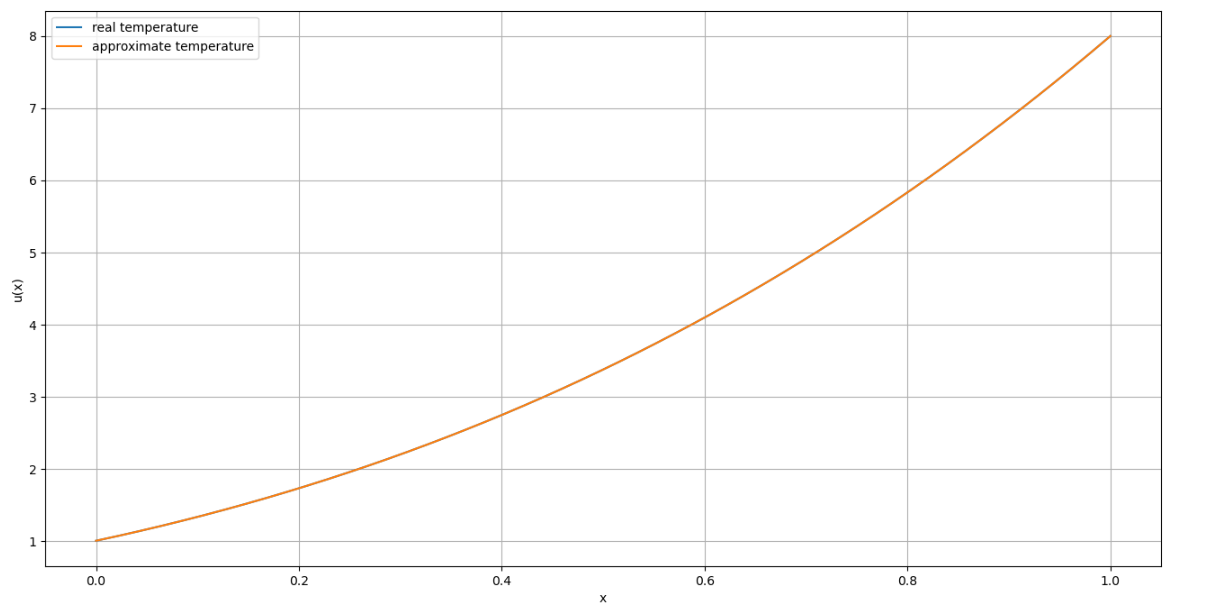
\includegraphics[width=1\linewidth]{image1.png}
\end{figure}
    
    Графики получились идентичными, для того, чтобы в этом убедиться,
посчитаем средний квадрат ошибки, который вычисляется следующим образом:
\[MSE=\frac{1}{N} \sum_{i=0}^N u(x_i)-\hat{u}(x_i),\] где $u(x_i) -$ точное решение, $\hat{u}(x_i) -$ приближенное решение.

    \begin{tcolorbox}[breakable, size=fbox, boxrule=1pt, pad at break*=1mm,colback=cellbackground, colframe=cellborder]
\prompt{In}{incolor}{6}{\boxspacing}
\begin{Verbatim}[commandchars=\\\{\}]
\PY{n}{mean\PYZus{}squared\PYZus{}error}\PY{p}{(}\PY{n}{u}\PY{p}{(}\PY{n}{x}\PY{p}{)}\PY{p}{,} \PY{n}{u\PYZus{}approx}\PY{p}{)}
\end{Verbatim}
\end{tcolorbox}

            \begin{tcolorbox}[breakable, size=fbox, boxrule=.5pt, pad at break*=1mm, opacityfill=0]
\prompt{Out}{outcolor}{6}{\boxspacing}
\begin{Verbatim}[commandchars=\\\{\}]
7.600835806367376e-25
\end{Verbatim}
\end{tcolorbox}
        
    И правда, ошибка у нас равна крайне малому значению, что позволяет
сделать вывод о том, что решение, полученное методом прогонки является
достаточно качественным.

    \subsubsection*{Метод прогонки для пункта
2.}\label{ux43cux435ux442ux43eux434-ux43fux440ux43eux433ux43eux43dux43aux438-ux434ux43bux44f-ux43fux443ux43dux43aux442ux430-2.}

Внесем все полученные коэффициенты, используемые в разностной схеме,
полученной методом баланса.

    \begin{tcolorbox}[breakable, size=fbox, boxrule=1pt, pad at break*=1mm,colback=cellbackground, colframe=cellborder]
\prompt{In}{incolor}{18}{\boxspacing}
\begin{Verbatim}[commandchars=\\\{\}]
\PY{k}{def} \PY{n+nf}{d\PYZus{}i}\PY{p}{(}\PY{n}{x}\PY{p}{,} \PY{n}{h}\PY{p}{)}\PY{p}{:}
    \PY{k}{return} \PY{o}{\PYZhy{}}\PY{l+m+mi}{7} \PY{o}{/} \PY{n}{h} \PY{o}{*} \PY{p}{(}\PY{l+m+mi}{1} \PY{o}{/} \PY{p}{(}\PY{n}{x} \PY{o}{+} \PY{n}{h} \PY{o}{/} \PY{l+m+mi}{2} \PY{o}{+} \PY{l+m+mi}{1}\PY{p}{)} \PY{o}{\PYZhy{}} \PY{l+m+mi}{1} \PY{o}{/} \PY{p}{(}\PY{n}{x} \PY{o}{\PYZhy{}} \PY{n}{h} \PY{o}{/} \PY{l+m+mi}{2} \PY{o}{+} \PY{l+m+mi}{1}\PY{p}{)}\PY{p}{)} 

\PY{k}{def} \PY{n+nf}{phi\PYZus{}i}\PY{p}{(}\PY{n}{x}\PY{p}{,} \PY{n}{h}\PY{p}{)}\PY{p}{:}
    \PY{k}{return} \PY{l+m+mi}{1} \PY{o}{/} \PY{n}{h} \PY{o}{*} \PY{p}{(}\PY{n}{x} \PY{o}{\PYZhy{}} \PY{n}{h} \PY{o}{/} \PY{l+m+mi}{2} \PY{o}{\PYZhy{}} \PY{n}{x} \PY{o}{\PYZhy{}} \PY{n}{h} \PY{o}{/} \PY{l+m+mi}{2} \PY{o}{+} \PY{p}{(}\PY{p}{(}\PY{n}{x} \PY{o}{\PYZhy{}} \PY{n}{h} \PY{o}{/} \PY{l+m+mi}{2}\PY{p}{)}\PY{o}{*}\PY{o}{*}\PY{l+m+mi}{2} \PY{o}{\PYZhy{}} \PY{p}{(}\PY{n}{x} \PY{o}{+} \PY{n}{h} \PY{o}{/} \PY{l+m+mi}{2}\PY{p}{)}\PY{o}{*}\PY{o}{*}\PY{l+m+mi}{2}\PY{p}{)} \PY{o}{/} \PY{l+m+mi}{2}\PY{p}{)}
\end{Verbatim}
\end{tcolorbox}

    Зададим коэффициенты метода прогонки

    \begin{tcolorbox}[breakable, size=fbox, boxrule=1pt, pad at break*=1mm,colback=cellbackground, colframe=cellborder]
\prompt{In}{incolor}{42}{\boxspacing}
\begin{Verbatim}[commandchars=\\\{\}]
\PY{n}{alpha} \PY{o}{=} \PY{p}{[}\PY{l+m+mi}{0}\PY{p}{]}
\PY{n}{gamma} \PY{o}{=} \PY{p}{[}\PY{l+m+mi}{1}\PY{p}{]}
\PY{n}{beta} \PY{o}{=} \PY{p}{[}\PY{l+m+mi}{0}\PY{p}{]}
\PY{n}{g} \PY{o}{=} \PY{p}{[}\PY{n}{A}\PY{p}{]}

\PY{k}{for} \PY{n}{i} \PY{o+ow}{in} \PY{n+nb}{range}\PY{p}{(}\PY{l+m+mi}{1}\PY{p}{,} \PY{n}{N}\PY{p}{)}\PY{p}{:}
    \PY{n}{alpha}\PY{o}{.}\PY{n}{append}\PY{p}{(}\PY{l+m+mi}{1} \PY{o}{/} \PY{n}{h}\PY{o}{*}\PY{o}{*}\PY{l+m+mi}{2}\PY{p}{)}
    \PY{n}{gamma}\PY{o}{.}\PY{n}{append}\PY{p}{(}\PY{o}{\PYZhy{}} \PY{p}{(}\PY{l+m+mi}{2}\PY{p}{)} \PY{o}{/} \PY{n}{h}\PY{o}{*}\PY{o}{*}\PY{l+m+mi}{2} \PY{o}{\PYZhy{}} \PY{n}{d\PYZus{}i}\PY{p}{(}\PY{n}{x}\PY{p}{[}\PY{n}{i}\PY{p}{]}\PY{p}{,} \PY{n}{h}\PY{p}{)}\PY{p}{)}
    \PY{n}{beta}\PY{o}{.}\PY{n}{append}\PY{p}{(}\PY{l+m+mi}{1} \PY{o}{/} \PY{n}{h}\PY{o}{*}\PY{o}{*}\PY{l+m+mi}{2}\PY{p}{)}
    \PY{n}{g}\PY{o}{.}\PY{n}{append}\PY{p}{(}\PY{o}{\PYZhy{}}\PY{n}{phi\PYZus{}i}\PY{p}{(}\PY{n}{x}\PY{p}{[}\PY{n}{i}\PY{p}{]}\PY{p}{,} \PY{n}{h}\PY{p}{)}\PY{p}{)}

\PY{n}{alpha}\PY{o}{.}\PY{n}{append}\PY{p}{(}\PY{l+m+mi}{0}\PY{p}{)}
\PY{n}{gamma}\PY{o}{.}\PY{n}{append}\PY{p}{(}\PY{l+m+mi}{1}\PY{p}{)}
\PY{n}{beta}\PY{o}{.}\PY{n}{append}\PY{p}{(}\PY{l+m+mi}{0}\PY{p}{)}
\PY{n}{g}\PY{o}{.}\PY{n}{append}\PY{p}{(}\PY{n}{B}\PY{p}{)}
\end{Verbatim}
\end{tcolorbox}

    Перейдем к визуализации.

    \begin{tcolorbox}[breakable, size=fbox, boxrule=1pt, pad at break*=1mm,colback=cellbackground, colframe=cellborder]
\prompt{In}{incolor}{43}{\boxspacing}
\begin{Verbatim}[commandchars=\\\{\}]
\PY{n}{u\PYZus{}approx} \PY{o}{=} \PY{n}{tridiagonal\PYZus{}algorithm}\PY{p}{(}\PY{n}{alpha}\PY{p}{,} \PY{n}{beta}\PY{p}{,} \PY{n}{gamma}\PY{p}{,} \PY{n}{g}\PY{p}{)}

\PY{n}{plt}\PY{o}{.}\PY{n}{figure}\PY{p}{(}\PY{n}{figsize}\PY{o}{=}\PY{p}{(}\PY{l+m+mi}{16}\PY{p}{,} \PY{l+m+mi}{8}\PY{p}{)}\PY{p}{)}
\PY{n}{plt}\PY{o}{.}\PY{n}{plot}\PY{p}{(}\PY{n}{x}\PY{p}{,} \PY{n}{u}\PY{p}{(}\PY{n}{x}\PY{p}{)}\PY{p}{,} \PY{n}{label}\PY{o}{=}\PY{l+s+s1}{\PYZsq{}}\PY{l+s+s1}{real temperature}\PY{l+s+s1}{\PYZsq{}}\PY{p}{)}
\PY{n}{plt}\PY{o}{.}\PY{n}{plot}\PY{p}{(}\PY{n}{x}\PY{p}{,} \PY{n}{u\PYZus{}approx}\PY{p}{,} \PY{n}{label}\PY{o}{=}\PY{l+s+s1}{\PYZsq{}}\PY{l+s+s1}{approximate temperature}\PY{l+s+s1}{\PYZsq{}}\PY{p}{)}
\PY{n}{plt}\PY{o}{.}\PY{n}{grid}\PY{p}{(}\PY{k+kc}{True}\PY{p}{)}
\PY{n}{plt}\PY{o}{.}\PY{n}{xlabel}\PY{p}{(}\PY{l+s+s1}{\PYZsq{}}\PY{l+s+s1}{x}\PY{l+s+s1}{\PYZsq{}}\PY{p}{)}
\PY{n}{plt}\PY{o}{.}\PY{n}{ylabel}\PY{p}{(}\PY{l+s+s1}{\PYZsq{}}\PY{l+s+s1}{u(x)}\PY{l+s+s1}{\PYZsq{}}\PY{p}{)}
\PY{n}{plt}\PY{o}{.}\PY{n}{legend}\PY{p}{(}\PY{p}{)}
\PY{n}{plt}\PY{o}{.}\PY{n}{show}\PY{p}{(}\PY{p}{)}
\end{Verbatim}
\end{tcolorbox}

\begin{figure}
    \centering
    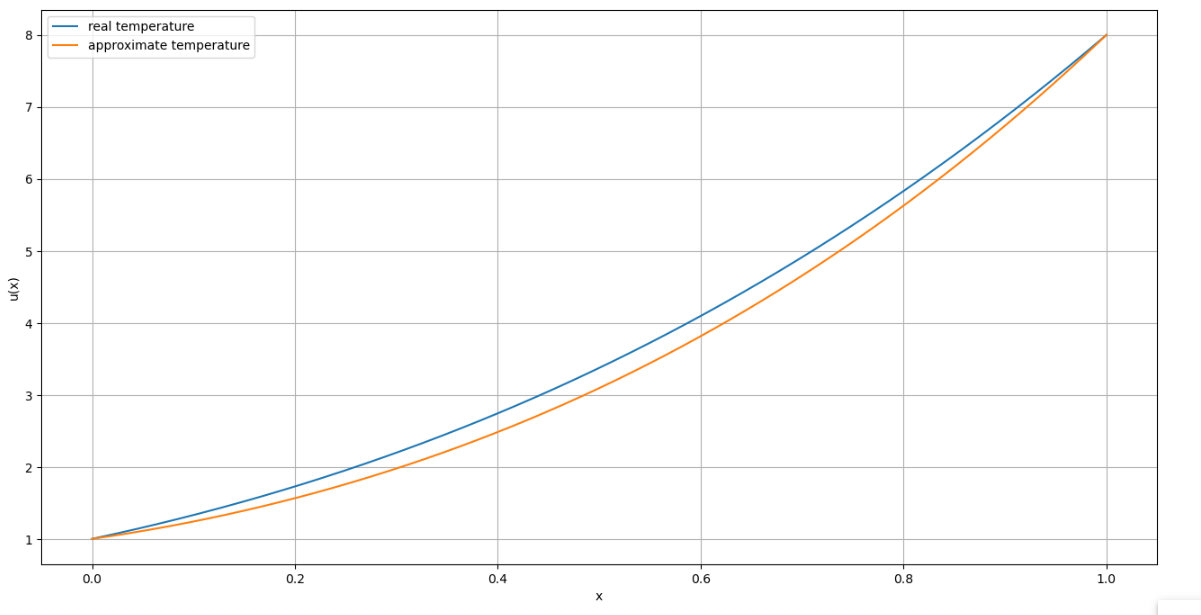
\includegraphics[width=1\linewidth]{image2.png}
\end{figure}
    
    Видно, что кривые немного отличаются. Для того, чтобы оценить эту
неточность, посчитаем, анлогично первому пункту, MSE.

    \begin{tcolorbox}[breakable, size=fbox, boxrule=1pt, pad at break*=1mm,colback=cellbackground, colframe=cellborder]
\prompt{In}{incolor}{45}{\boxspacing}
\begin{Verbatim}[commandchars=\\\{\}]
\PY{n}{mean\PYZus{}squared\PYZus{}error}\PY{p}{(}\PY{n}{u}\PY{p}{(}\PY{n}{x}\PY{p}{)}\PY{p}{,} \PY{n}{u\PYZus{}approx}\PY{p}{)}
\end{Verbatim}
\end{tcolorbox}

            \begin{tcolorbox}[breakable, size=fbox, boxrule=.5pt, pad at break*=1mm, opacityfill=0]
\prompt{Out}{outcolor}{45}{\boxspacing}
\begin{Verbatim}[commandchars=\\\{\}]
0.04293360244618271
\end{Verbatim}
\end{tcolorbox}
        
    Из этого можно сделать вывод о том, что метод прогонки для разностной
схемы, построенной методом баланса, работает неплохо, но не идеально.
\subsubsection*{Вывод}
По полученным результатам можно сделать вывод, что метод прогонки для пунка 1 позволяет найти более точное решение, чем для пункта 2. На это указывает как график, так и выбранная метрика.

    % Add a bibliography block to the postdoc
    
    
    
\end{document}